\section{Results}
\label{sec:results}

\subsection{The convention decides the ranking}
\label{sec:ranking}

Table~\ref{tab:main} scores one set of runs four ways. The predictions are
identical down the row; only the function applied to them changes.

\begin{table}[t]
\centering
\begin{tabular}{lccccc}
\toprule
 & \multicolumn{4}{c}{F1 under each convention} & \\
\cmidrule(lr){2-5}
Model, policy & Point-wise & Composite & Range & Point-adj. & Alarm rate \\
\midrule
HST, never & 0.377 \ci{0.346}{0.409} & 0.531 \ci{0.512}{0.549} & 0.008 \ci{0.008}{0.009} & 0.742 \ci{0.722}{0.761} & 0.380 \\
HST, online & 0.314 \ci{0.292}{0.334} & 0.523 \ci{0.516}{0.529} & 0.007 \ci{0.007}{0.007} & 0.794 \ci{0.777}{0.811} & 0.278 \\
HST, periodic & 0.517 \ci{0.509}{0.527} & 0.606 \ci{0.599}{0.613} & 0.045 \ci{0.029}{0.067} & 0.707 \ci{0.704}{0.710} & 0.505 \\
HST, drift & 0.477 \ci{0.471}{0.483} & 0.576 \ci{0.570}{0.581} & 0.024 \ci{0.022}{0.027} & 0.700 \ci{0.696}{0.703} & 0.496 \\
iForest, never & 0.514 \ci{0.513}{0.515} & 0.514 \ci{0.513}{0.515} & 0.026 \ci{0.006}{0.052} & 0.514 \ci{0.513}{0.515} & 0.995 \\
iForest, periodic & 0.538 \ci{0.536}{0.539} & 0.548 \ci{0.545}{0.550} & 0.198 \ci{0.184}{0.213} & 0.563 \ci{0.560}{0.566} & 0.857 \\
iForest, drift & 0.539 \ci{0.537}{0.541} & 0.550 \ci{0.548}{0.553} & 0.114 \ci{0.106}{0.124} & 0.569 \ci{0.565}{0.572} & 0.842 \\
LOF, never & 0.514 & 0.514 & 0.001 & 0.514 & 0.996 \\
OC-SVM, never & 0.513 & 0.513 & 0.002 & 0.513 & 0.998 \\
MCD, never & 0.513 \ci{0.513}{0.513} & 0.513 \ci{0.513}{0.513} & 0.001 \ci{0.001}{0.001} & 0.513 \ci{0.513}{0.513} & 0.997 \\
\midrule
Flag everything & 0.512 & 0.512 & 0.045 & 0.512 & 1.000 \\
\bottomrule
\end{tabular}

\caption{Every strategy on the labelled SKAB stream, scored under four published
conventions. Means over \NSeeds{} seeds with 95\% bootstrap intervals; a cell
with no interval is an estimator that is deterministic given the data. The last
row is the score obtained by flagging every single row, which any result has to
clear to mean anything.}
\label{tab:main}
\end{table}

The four conventions produce \NDistinctWinners{} different winners.
Point-wise F1 puts \BestPoint{} first at \BestPointVal{}; the composite
F-score puts \BestComposite{} first at \BestCompositeVal{}; range-based scoring
puts \BestRange{} first at \BestRangeVal{}. \NRankChanges{} of \NStrategies{}
strategies change rank between point-wise and composite scoring, and the largest
single move is \MaxRankJump{} places. \MoverName{} is the clearest case: it
places \MoverPointRank{} under point-wise F1 and \MoverCompositeRank{} under
the composite score, on the same flags.

Figure~\ref{fig:ranking} shows why, and Figure~\ref{fig:rankflip} draws the
same reordering as a bump chart. Point-wise recall rewards a detector for
flagging every row of a long fault, and SKAB's faults average about 390 rows, so
a detector that flags each fault sparsely is punished for exactly the behaviour
an operator wants. Event-level recall asks instead whether each fault was
noticed at all. Neither is wrong. They are answers to different questions, and
which one is asked decides the ranking.

\begin{figure}[t]
\centering
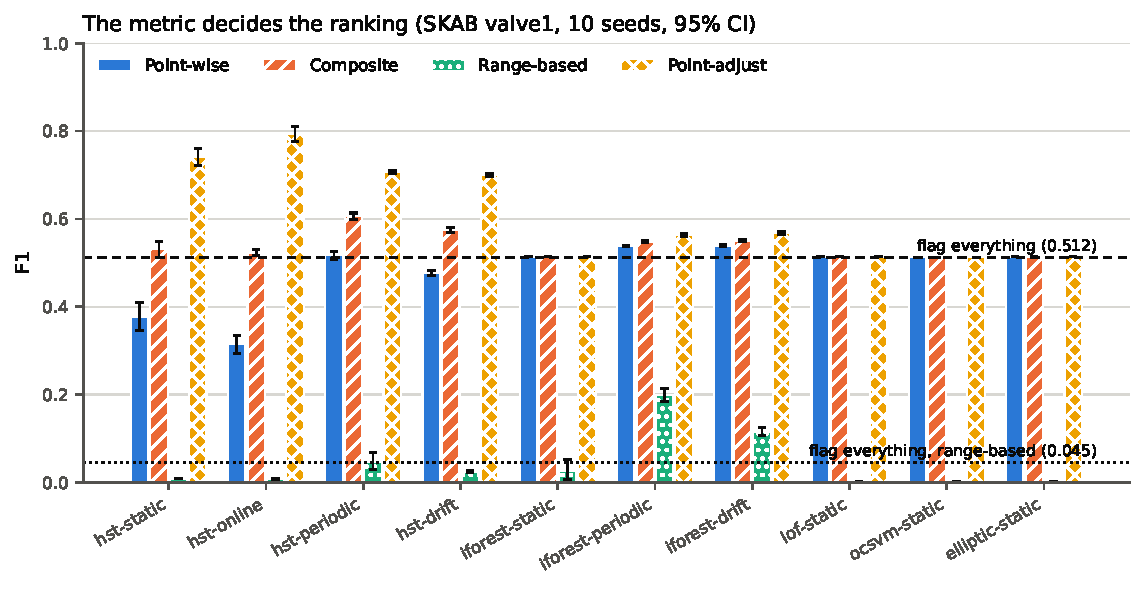
\includegraphics[width=\textwidth]{../results/figures/paper/metric_ranking.pdf}
\caption{The same runs under four scoring conventions, with 95\% bootstrap
intervals over \NSeeds{} seeds. The dashed line is the flag-everything
baseline.}
\label{fig:ranking}
\end{figure}

\begin{figure}[t]
\centering
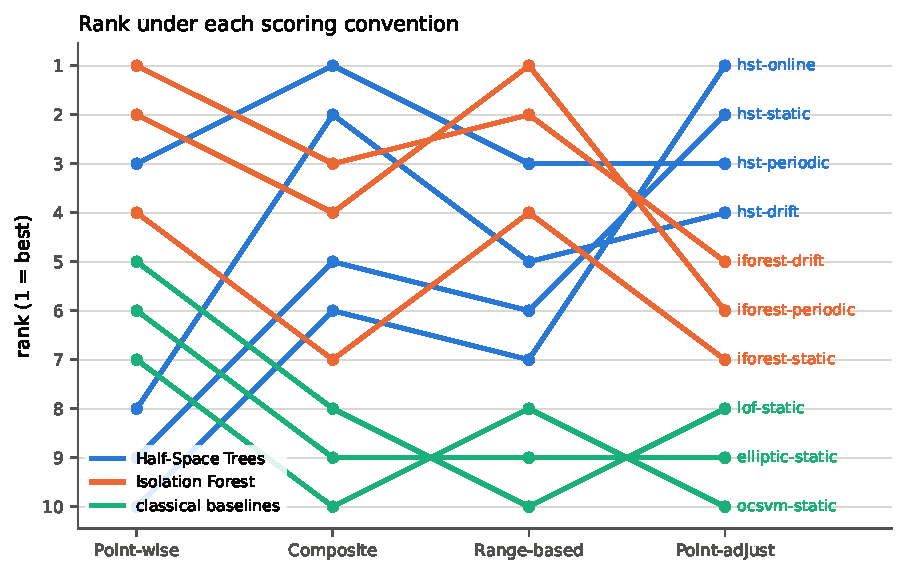
\includegraphics[width=0.72\textwidth]{../results/figures/paper/rank_flip.pdf}
\caption{Rank of each strategy under each convention. Colour is the model
family; each line is labelled with its strategy, and a line drawn faintly is one
whose rank is the same under all four conventions.}
\label{fig:rankflip}
\end{figure}

Point-adjust is included to show what it does to the table. We do not rely on it.
It credits an entire fault block for one flagged row, which on 390-row blocks
inflates every strategy at once. \citet{kim2022rigorous} showed that this lets
random predictions outscore trained models, and our test suite reproduces that
failure directly: two flags placed in a 300-row stream reach a point-adjust
recall of 1.0 against a point-wise recall of 0.01.

The last column of Table~\ref{tab:main} is the one to read first.
\NBeatPoint{} of \NStrategies{} strategies clear the flag-everything baseline
under point-wise scoring and \NBeatComposite{} clear it under the composite
score. A detector that flags 99\% of rows scores near the baseline by
construction, and several of the static baselines do exactly that.

Range-based scoring moves the baseline as well as the detectors, and it is
worth saying where it lands. Flagging every row produces one predicted range
spanning the stream, so its precision is divided by the number of true events
that range swallows, and the trivial baseline drops to \FlagAllRange{}.
Against that, \NBeatRange{} of \NStrategies{} strategies clear it. The
detectors are charged in the opposite direction: a permissive policy emits
thousands of short predicted ranges across each fault, and the cardinality
factor bills it for every fragment. Fragmentation is invisible to the other
three conventions and decisive under this one.

\subsection{Model against policy}
\label{sec:factorial}

The usual presentation of this comparison contrasts a static Isolation Forest
against an adaptive Half-Space Trees model, which confounds the two factors.
Figure~\ref{fig:factorial} crosses them.

\begin{figure}[t]
\centering
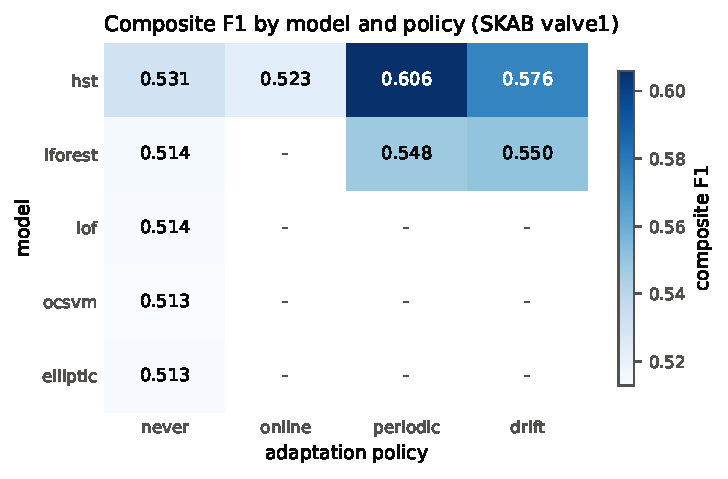
\includegraphics[width=0.62\textwidth]{../results/figures/paper/factorial.pdf}
\caption{Composite F1 by model and adaptation policy. The three classical
detectors appear only under \emph{never}: none supports an incremental update,
so for them adaptation could only mean a refit.}
\label{fig:factorial}
\end{figure}

Reading down a column separates the model from the policy, and reading across a
row separates the policy from the model. Both factors move the score, and the
policy moves it further: under the composite view the spread across policies
within Half-Space Trees is wider than the spread across models within the
\emph{never} column. The three classical baselines sit at the bottom of that
column together, all of them flagging over 99\% of rows, which is the same
failure the static Isolation Forest shows and not a quirk of one model.

The MCD estimator is worth a note, because it is the one baseline that had to
be nursed. It assumes the normal data forms one elliptical cloud, which SKAB's
multi-regime stream violates, and \texttt{scikit-learn} emits a determinant
warning on nearly every fit. On one NAB series it fails outright: 859 of the
1{,}000 warm-up rows there are exactly 0.0, so the robust support it selects is
entirely constant and the covariance is singular. We widen the support fraction
until it fits and record that we did. Both facts are reported because a
baseline that struggles for a stated structural reason is more useful than one
quietly dropped.

\subsection{Does the ranking survive the data?}
\label{sec:replication}

Seeds test whether a gap survives the randomness. They do not test whether it
survives a different recording, and on this data that is the harder question.
Figure~\ref{fig:segments} scores every strategy separately on each of the
\NRecordings{} source recordings that contain a fault.

\begin{figure}[t]
\centering
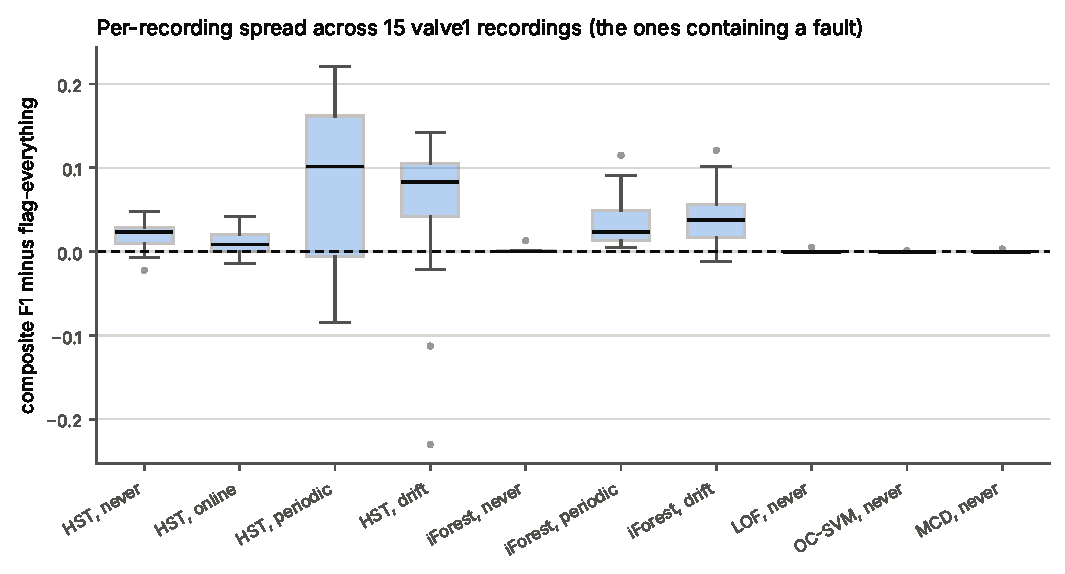
\includegraphics[width=\textwidth]{../results/figures/paper/segment_spread.pdf}
\caption{Composite F1 minus the flag-everything baseline, one point per source
recording, averaged over seeds. A box straddling zero is a strategy that does
not reliably beat flagging everything on an arbitrary recording.}
\label{fig:segments}
\end{figure}

Table~\ref{tab:significance} reports the paired comparisons the paper makes,
over both units. Of \NComparisons{} comparisons on the labelled stream,
\NSignificant{} survive Holm correction.

\begin{table}[t]
\centering
\small
\begin{tabular}{llcccc}
\toprule
Comparison & Metric & Unit & Mean diff. [95\% CI] & $p$ & Holm \\
\midrule
HST, periodic vs.\ HST, never & point & seed & $+0.140$ $[+0.109, +0.169]$ & 0.0020 & \yes \\
HST, drift vs.\ HST, never & point & seed & $+0.100$ $[+0.067, +0.131]$ & 0.0020 & \yes \\
HST, periodic vs.\ HST, drift & point & seed & $+0.040$ $[+0.035, +0.045]$ & 0.0020 & \yes \\
HST, periodic vs.\ HST, online & point & seed & $+0.203$ $[+0.184, +0.221]$ & 0.0020 & \yes \\
iForest, periodic vs.\ iForest, never & point & seed & $+0.024$ $[+0.023, +0.025]$ & 0.0020 & \yes \\
iForest, drift vs.\ iForest, never & point & seed & $+0.025$ $[+0.023, +0.026]$ & 0.0020 & \yes \\
HST, periodic vs.\ iForest, periodic & point & seed & $-0.021$ $[-0.029, -0.012]$ & 0.0059 & \yes \\
HST, never vs.\ iForest, never & point & seed & $-0.137$ $[-0.168, -0.104]$ & 0.0020 & \yes \\
HST, periodic vs.\ HST, never & point & segment & $+0.134$ $[+0.066, +0.198]$ & 0.0067 & \yes \\
HST, drift vs.\ HST, never & point & segment & $+0.085$ $[+0.016, +0.147]$ & 0.0353 & \no \\
HST, periodic vs.\ HST, drift & point & segment & $+0.049$ $[+0.004, +0.097]$ & 0.0554 & \no \\
HST, periodic vs.\ HST, online & point & segment & $+0.197$ $[+0.131, +0.260]$ & 0.0001 & \yes \\
iForest, periodic vs.\ iForest, never & point & segment & $+0.025$ $[+0.011, +0.041]$ & 0.0020 & \yes \\
iForest, drift vs.\ iForest, never & point & segment & $+0.026$ $[+0.008, +0.045]$ & 0.0151 & \no \\
HST, periodic vs.\ iForest, periodic & point & segment & $-0.029$ $[-0.086, +0.026]$ & 0.3894 & \no \\
HST, never vs.\ iForest, never & point & segment & $-0.138$ $[-0.146, -0.130]$ & 0.0001 & \yes \\
\midrule
HST, periodic vs.\ HST, never & composite & seed & $+0.075$ $[+0.058, +0.092]$ & 0.0020 & \yes \\
HST, drift vs.\ HST, never & composite & seed & $+0.045$ $[+0.027, +0.063]$ & 0.0020 & \yes \\
HST, periodic vs.\ HST, drift & composite & seed & $+0.030$ $[+0.026, +0.035]$ & 0.0020 & \yes \\
HST, periodic vs.\ HST, online & composite & seed & $+0.083$ $[+0.077, +0.089]$ & 0.0020 & \yes \\
iForest, periodic vs.\ iForest, never & composite & seed & $+0.033$ $[+0.032, +0.035]$ & 0.0020 & \yes \\
iForest, drift vs.\ iForest, never & composite & seed & $+0.036$ $[+0.034, +0.038]$ & 0.0020 & \yes \\
HST, periodic vs.\ iForest, periodic & composite & seed & $+0.058$ $[+0.052, +0.066]$ & 0.0020 & \yes \\
HST, never vs.\ iForest, never & composite & seed & $+0.017$ $[-0.002, +0.035]$ & 0.1934 & \no \\
HST, periodic vs.\ HST, never & composite & segment & $+0.064$ $[+0.010, +0.114]$ & 0.0479 & \no \\
HST, drift vs.\ HST, never & composite & segment & $+0.030$ $[-0.028, +0.078]$ & 0.1070 & \no \\
HST, periodic vs.\ HST, drift & composite & segment & $+0.034$ $[-0.016, +0.082]$ & 0.1876 & \no \\
HST, periodic vs.\ HST, online & composite & segment & $+0.072$ $[+0.021, +0.119]$ & 0.0256 & \no \\
iForest, periodic vs.\ iForest, never & composite & segment & $+0.036$ $[+0.021, +0.055]$ & 0.0002 & \yes \\
iForest, drift vs.\ iForest, never & composite & segment & $+0.038$ $[+0.021, +0.058]$ & 0.0006 & \yes \\
HST, periodic vs.\ iForest, periodic & composite & segment & $+0.045$ $[-0.003, +0.089]$ & 0.1070 & \no \\
HST, never vs.\ iForest, never & composite & segment & $+0.017$ $[+0.008, +0.025]$ & 0.0026 & \yes \\
\bottomrule
\end{tabular}

\caption{Paired comparisons on the labelled stream, over seeds and over source
recordings. Differences are the first strategy minus the second, with 95\%
bootstrap intervals. $p$ is a two-sided Wilcoxon signed-rank test; the last
column is the decision after Holm correction within the stream. Point-wise and
composite scoring are shown; the range-based comparisons are counted in the
totals quoted above and listed in full in \texttt{results/significance.csv}.}
\label{tab:significance}
\end{table}

The between-recording spread is the reason we consider the single-run tables
this project started with to have been unsupportable. It is wide enough that a
gap of a few hundredths, reported from one run, carries no information about
which policy to deploy.

It also complicates the aggregate ranking. \BestComposite{}, which wins
Table~\ref{tab:main} on the mean, fails to beat the trivial baseline on
\BestCompositeLosses{} of the \NRecordings{} recordings, and its interquartile
range in Figure~\ref{fig:segments} straddles zero. \SteadiestName{} scores
lower on average but fails on \SteadiestLosses{} of them, with an interquartile
range entirely above zero. Which of the two an operator should prefer depends on
whether they are averaging over many streams or deploying on one, and the mean
in the headline table cannot answer that.

\subsection{Drift detectors and detection timing}
\label{sec:timing}

The injected streams are where timing can be measured, because the change point
is known to the row and nothing in the stream is genuinely anomalous.
Table~\ref{tab:detectors} reports the delay at a 3\,sd shift.

\begin{table}[t]
\centering
\begin{tabular}{lccccc}
\toprule
Detector & sudden & incremental & gradual & recurring & False alarms / 1k \\
\midrule
\texttt{adwin} & 9 & 181 & 258 \ci{219}{296} & 20 & 1.92 \\
\texttt{adwin\_meanvar} & 9 & 181 & 104 \ci{85}{130} & 20 & 1.99 \\
\texttt{adwin\_var} & 9 & -- & 104 \ci{72}{130} & 30 & 0.29 \\
\texttt{kswin} & 107 \ci{59}{136} & 176 \ci{102}{242} & 202 \ci{90}{338} & 124 \ci{58}{194} & 2.77 \\
\texttt{pagehinkley} & 6 & 255 & 193 \ci{173}{212} & 5 & 1.53 \\
\bottomrule
\end{tabular}

\caption{Mean detection delay in rows at a 3\,sd shift, by drift shape, with 95\%
bootstrap intervals over seeds. A dash is a detector that never fired on that
shape. The last column is false alarms per 1{,}000 steps, averaged over shapes
and magnitudes.}
\label{tab:detectors}
\end{table}

\begin{figure}[t]
\centering
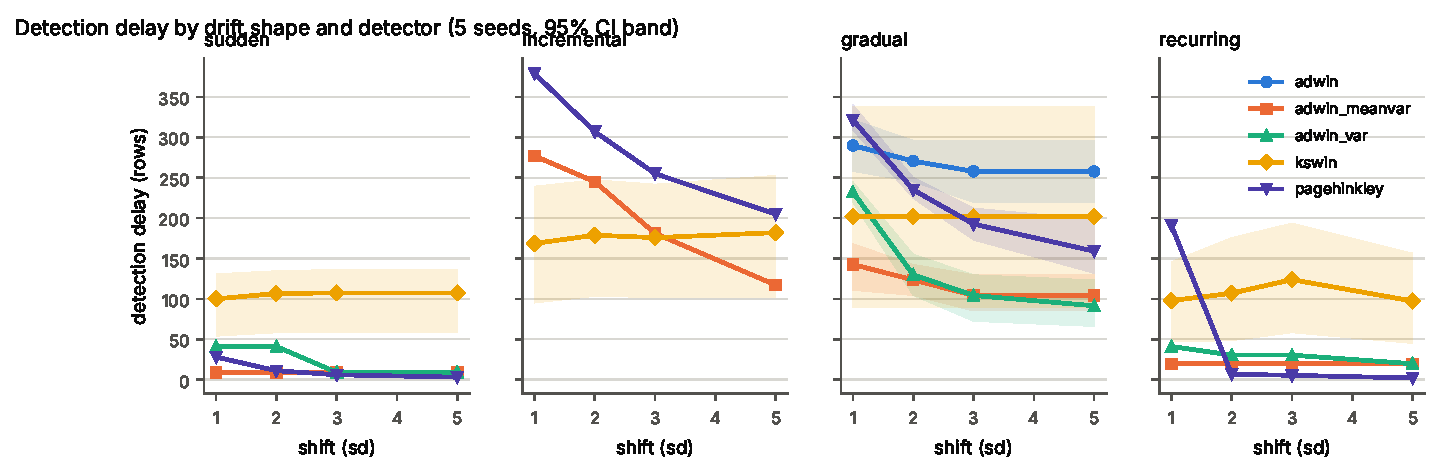
\includegraphics[width=\textwidth]{../results/figures/paper/detector_delay.pdf}
\caption{Detection delay against shift magnitude, one panel per drift shape.
Bands are 95\% bootstrap intervals over seeds.}
\label{fig:delay}
\end{figure}

Figure~\ref{fig:delay} plots the same measurement against magnitude. Two
shapes separate the detectors. A sudden step is caught quickly by anything that
watches the mean. Gradual drift, where the two regimes interleave before the
mean has moved, is the case a location detector cannot see: early in the
transition individual rows flip between the old and new regime, so the signal
grows spiky before its level changes. Feeding ADWIN the trailing \emph{variance}
of the monitored statistic, in place of its level, reacts to that. It cuts the
gradual delay by more than half, and it pays for that by going blind to a smooth
ramp, which shifts the mean without changing the spread: on the incremental
shape it never fires at all, at any magnitude. Running a mean ADWIN and a
variance ADWIN together and firing when either does recovers every shape and
keeps the better gradual delay.

Page-Hinkley was added to this comparison as a third opinion and turned out to
be the most interesting entry in the table. It is the quickest of the five on
both the sudden and the recurring shapes, and it raises fewer false alarms than
ADWIN while doing it. What it gives up is the incremental ramp, where it is the
slowest detector that fires at all: a cumulative sum needs the deviation to
accumulate, and a slow ramp supplies it slowly. That is a clean trade and not a
defect, and it is the kind of thing a single-detector study cannot see.
KSWIN is the one detector we would not recommend from these numbers: it is
slower than ADWIN on every shape and raises the most false alarms of the five.

The false-alarm column has to be read with Section~\ref{sec:limitations} in mind.
SKAB's anomaly-free recording is not stationary, so an unknown share of those
firings are the detector correctly noticing real process change.

\subsection{Transferring the calibration}
\label{sec:transfer}

Everything above is tuned on one industrial rig, which invites the objection
that the settings are fitted to it. Table~\ref{tab:transfer} applies the SKAB
threshold to \NNabSeries{} NAB series unchanged. NAB is univariate where SKAB
has eight sensors, and roughly 10\% anomalous where SKAB is \BaseRate\%, so it
breaks a transferred calibration in the ways that matter.

\begin{table}[t]
\centering
\small
\begin{tabular}{lccccc}
\toprule
NAB series & Best strategy & Flag-all & Point-wise F1 & Composite F1 & Beats \\
\midrule
ambient\_temperature & HST, periodic & 0.208 & 0.313 \ci{0.285}{0.338} & 0.543 \ci{0.463}{0.619} & \yes \\
cpu\_utilization\_asg & iForest, periodic & 0.162 & 0.338 \ci{0.317}{0.365} & 0.522 \ci{0.502}{0.546} & \yes \\
ec2\_request\_latency & HST, drift & 0.205 & 0.090 \ci{0.087}{0.093} & 0.376 \ci{0.363}{0.388} & \yes \\
machine\_temperature & MCD, never & 0.189 & 0.545 & 0.880 & \yes \\
nyc\_taxi & HST, online & 0.200 & 0.082 \ci{0.074}{0.093} & 0.388 \ci{0.327}{0.459} & \yes \\
rogue\_agent\_key\_updown & HST, drift & 0.219 & 0.040 \ci{0.040}{0.040} & 0.290 \ci{0.286}{0.294} & \yes \\
\bottomrule
\end{tabular}

\caption{NAB series with the SKAB threshold carried over unchanged, showing the
best strategy per series by composite F1. The flag-everything column is the
trivial baseline for that series.}
\label{tab:transfer}
\end{table}

\begin{figure}[t]
\centering
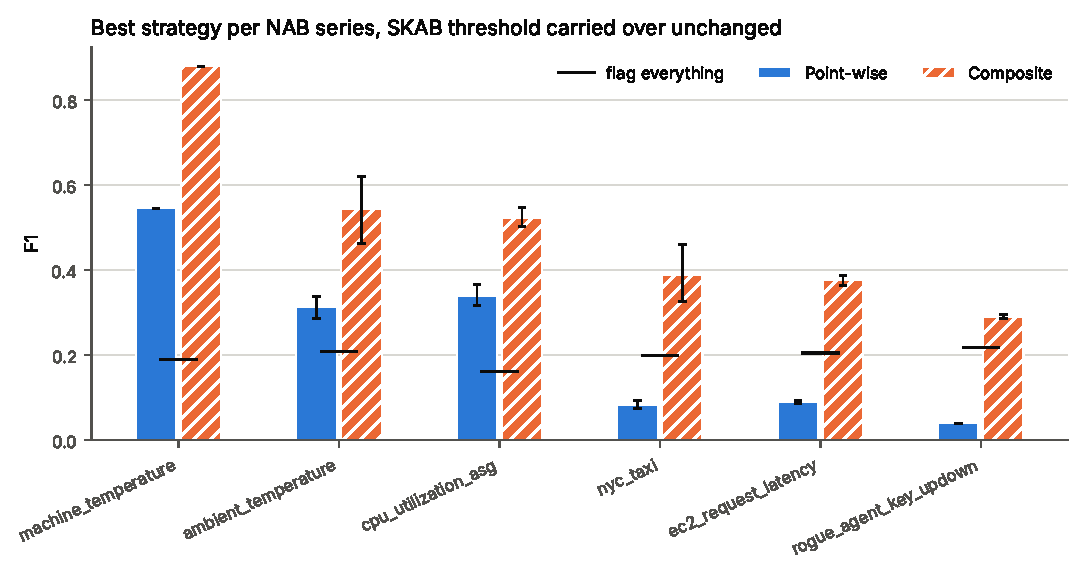
\includegraphics[width=\textwidth]{../results/figures/paper/transfer.pdf}
\caption{Best strategy per NAB series under point-wise and composite scoring,
with the trivial baseline marked.}
\label{fig:transfer}
\end{figure}

The metric effect reappears here and is larger than on SKAB
(Figure~\ref{fig:transfer}). Under point-wise
scoring the transferred setting beats the trivial baseline on
\NNabBeatsPoint{} of \NNabSeries{} series; under composite scoring it beats it
on \NNabBeatsComposite{}. NAB's anomalies are short and sparse, so point-wise
recall penalises a detector that flags a window without also flagging its
neighbourhood, which is the behaviour the composite score is built to credit.
The method carries across datasets in a way the point-wise numbers alone would
deny.

What does not carry is any particular strategy. \NNabDistinctWinners{}
different strategies take the top place across the \NNabSeries{} series, and
one of them is a classical static baseline. There is no ranking here to
transfer, only a method and a threshold that has to be set per deployment.

\subsection{Where event recall discriminates}
\label{sec:ucr}

Everything above is scored on data where the recall axis is nearly flat. On SKAB
every strategy catches every labelled event, so composite F1 is a ranking on
precision and nothing else. The UCR subset is here to supply the missing axis:
one anomaly per series, \NUcrSeries{} series, so a strategy either finds each
one or it does not.

\begin{table}[t]
\centering
\begin{tabular}{lccccc}
\toprule
Model, policy & Peak in window & Anomalies found & Composite F1 & Point-wise F1 & Alarm rate \\
\midrule
HST, never & 0.07 & 0.30 & 0.030 & 0.014 & 0.022 \\
HST, online & 0.06 & 0.42 & 0.023 & 0.013 & 0.032 \\
HST, periodic & 0.01 & 0.33 & 0.022 & 0.012 & 0.021 \\
HST, drift & 0.06 & 0.35 & 0.026 & 0.014 & 0.021 \\
iForest, never & 0.00 & 0.33 & 0.033 & 0.014 & 0.030 \\
iForest, periodic & 0.00 & 0.35 & 0.016 & 0.010 & 0.033 \\
iForest, drift & 0.01 & 0.26 & 0.019 & 0.011 & 0.029 \\
LOF, never & 0.12 & 0.50 & 0.030 & 0.021 & 0.046 \\
OC-SVM, never & 0.12 & 0.25 & 0.028 & 0.013 & 0.034 \\
MCD, never & 0.12 & 0.38 & 0.030 & 0.017 & 0.026 \\
\midrule
Flag everything & -- & 1.00 & 0.020 & 0.020 & 1.000 \\
\bottomrule
\end{tabular}

\caption{The UCR subset, averaged over \NUcrSeries{} series and \NSeeds{} seeds.
``Anomalies found'' is the proportion of series whose single anomaly the
strategy flagged at all, which is event-level recall when every series has
exactly one event. The trivial baseline finds every anomaly by definition and
pays for it in precision.}
\label{tab:ucr}
\end{table}

\begin{figure}[t]
\centering
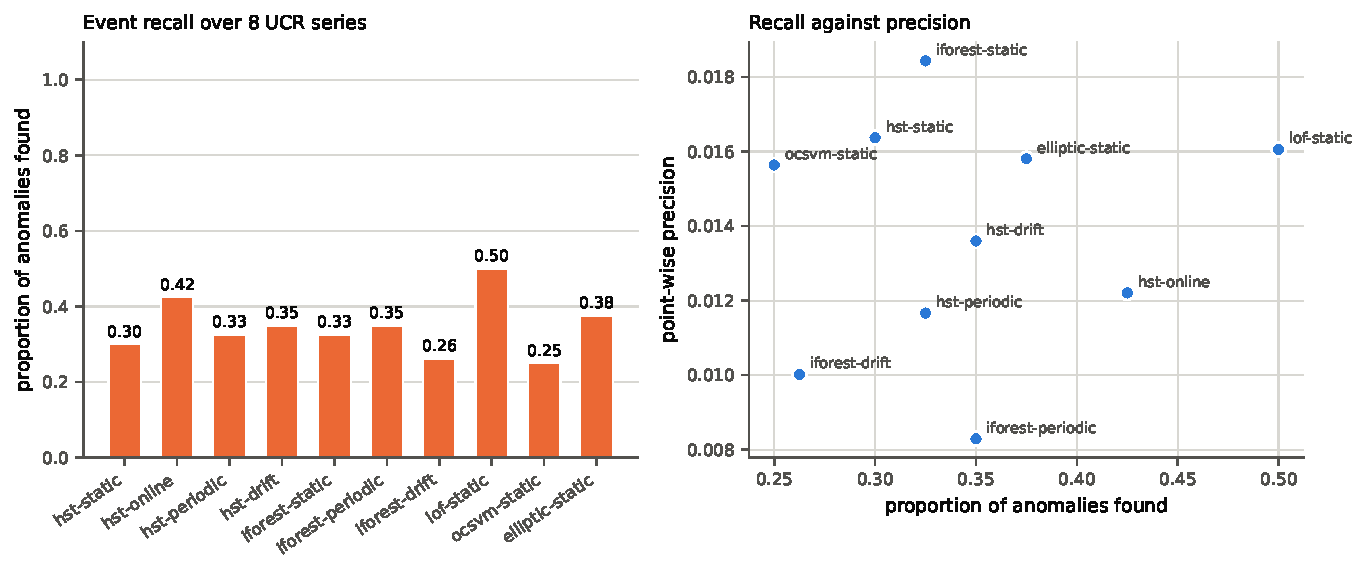
\includegraphics[width=\textwidth]{../results/figures/paper/ucr.pdf}
\caption{Left: the proportion of UCR anomalies each strategy found. Right: the
same quantity against point-wise precision, which is the trade the composite
score combines.}
\label{fig:ucr}
\end{figure}

The proportion of anomalies found (Figure~\ref{fig:ucr}) runs from
\WorstUcrFound{} for \WorstUcrName{} to \BestUcrFound{} for \BestUcrName{}, a
spread of \UcrRecallSpread{}. That spread is the first thing to note. It is a real
difference between strategies that SKAB cannot show at all and NAB shows only
partially, and it exists because the benchmark was built so a detector can miss.

The second thing to note is the level. The best strategy here finds
\BestUcrFound{} of the anomalies. Not one of the ten finds most of them, and
that is on a subset chosen for being short and tractable. Whatever these
policies are doing on SKAB, they are not solving this.

The base rate is \UcrBaseRate\%, which puts the trivial baseline at
\UcrFlagAll{} rather than the \FlagAll{} it reaches on SKAB. That is a much
lower bar and it is the bar a detector should face: where anomalies are genuinely
rare, flagging everything is obviously useless, and a benchmark on which it looks
competitive is the problem \citet{wu2023flawed} were describing.
\NUcrBeatComposite{} of \NStrategies{} strategies clear it under the composite
score and \NUcrBeatPoint{} point-wise, but the margins are small enough that
clearing it is not much of a claim.

\paragraph{The archive's own criterion.} Scoring UCR with a thresholded F1 is
not what its authors intended. They score a series as solved when the single
highest anomaly score falls inside the labelled window, and they argue for that
because it needs no threshold, so the cutoff stops being part of what is
measured. Substituting our own convention for theirs would be the exact move
this paper criticises, so Table~\ref{tab:ucr} reports both. Under the archive's
criterion the best strategy is \BestUcrTopOne{} at \BestUcrTopOneVal{}, the
worst manages \WorstUcrTopOneVal{}, and the average across all ten is
\MeanUcrTopOne{}. The two protocols do not even agree on a winner
(\TopOneAgreesWithComposite{}), which is the same disagreement this paper
documents between conventions, now reproduced between our scoring and the
dataset author's.

\paragraph{Adaptation does not help here.} The best composite score on this data
belongs to \BestUcrComposite{}, and the most anomalies are found by
\BestUcrName{}. Both are configured to \emph{\BestUcrPolicy{}}, and neither is
one of the \NUcrAdaptive{} adaptive configurations. On the benchmark built to be hard,
the question this paper is about stops mattering: the policies are separated by
less than the noise, and the classical static detectors are as good as anything
with a rebuild schedule. We report that because it is what the data says, and
because a paper that found adaptation mattered on two datasets and quietly left
out the third would be doing what its own introduction complains about.

\subsection{Sensitivity to the constants we chose}
\label{sec:ablation}

Three values in this design were picked by judgement: the warm-up length of
1{,}000 rows, the 750-step horizon within which a detection is credited to a
change point, and the 250-step cooldown after a detector fires.
Figure~\ref{fig:ablation} varies the first two.

\begin{figure}[t]
\centering
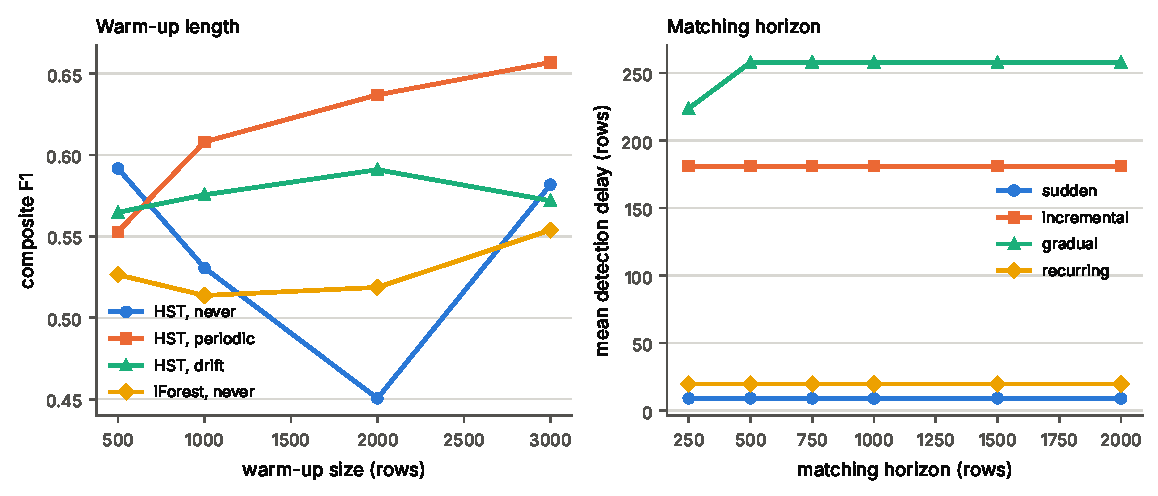
\includegraphics[width=\textwidth]{../results/figures/paper/ablation.pdf}
\caption{Left: composite F1 against warm-up length. Right: mean detection delay
against the matching horizon. Changing the warm-up also changes which rows are
scored, so the base rate moves with it; the raw counts are in
\texttt{results/ablation\_warmup.csv}.}
\label{fig:ablation}
\end{figure}

The matching horizon turns out not to be load-bearing. Past 500 steps the
mean delay is identical for every drift shape, and the gradual case is the
only one that moves at all between the shortest setting and the default. A
detection either lands close to the change point or does not land at all, so
the exact cut-off has little to decide.

Warm-up length is the constant that does matter, and it does not treat the
policies alike: the periodic schedule improves steadily as the warm-up
lengthens, while the drift-triggered one is flat and the static baseline moves
erratically. We report this as a sensitivity and not as a tuning result,
because changing the warm-up also changes which rows are scored, and on a
stream with unevenly spaced faults that moves the base rate underneath the
comparison. The per-setting base rates are in
\texttt{results/ablation\_warmup.csv}.

The cooldown behaves as it was designed to and buys less than expected. At the
two shortest settings the number of rebuilds is identical, which says the
detector's own firing spacing already exceeds them; only at the longest
setting does suppression bite hard enough to halve the rebuilds. None of the
conclusions above depends on the value we picked.

\subsection{Cost}
\label{sec:cost}

A streaming method that cannot keep up with the stream is not one.
Table~\ref{tab:cost} reports throughput on a single laptop core.

\begin{table}[t]
\centering
\begin{tabular}{lcc}
\toprule
Model, policy & Rows / second & Rebuilds \\
\midrule
HST, never & 19,325 & 0.0 \\
HST, online & 10,324 & 0.0 \\
HST, periodic & 2,530 & 17.0 \\
HST, drift & 947 & 35.0 \\
iForest, never & 29,714 & 0.0 \\
iForest, periodic & 2,430 & 17.0 \\
iForest, drift & 844 & 35.0 \\
LOF, never & 38,085 & 0.0 \\
OC-SVM, never & 129,212 & 0.0 \\
MCD, never & 34,839 & 0.0 \\
\bottomrule
\end{tabular}

\caption{Throughput and rebuild count on the labelled stream, averaged over
seeds. The static sklearn baselines score in vectorised blocks; the Half-Space
Trees implementation scores one observation at a time, which is the honest cost
of an online model in this library.}
\label{tab:cost}
\end{table}

The spread here is a property of the implementations, not of the algorithms:
Half-Space Trees is scored one observation at a time in \texttt{river}, while
the sklearn baselines are scored in vectorised blocks. It is reported because a
comparison that leaves cost out is incomplete. On this hardware the slowest
strategy, \SlowestModel{}, processes \SlowestRows{} rows per second against
\FastestRows{} for \FastestModel{}, a factor of about \SpeedRatio{}. Every
strategy here keeps up with anything a single sensor rig produces; the figure
starts to matter when one detector is run across thousands of streams at once.
